\documentclass[Main.tex]{subfiles}
\begin{document}
			\section{Measures of Influence} %1.16
		
		The impact of an observation, or a case with multiple obverations, on a regression fitting can be determined by the difference between the estimated regression coefficient of a model with all observations and the estimated coefficient when the particular observation is deleted. The measure DFBETA is the studentized value of this difference.
		
		
		\subsection{Overall Influence}
		An overall influence statistic measures the change in the objective function being minimized. For example, in
		OLS regression, the residual sums of squares serves that purpose. In linear mixed models fit by
		\index{maximum likelihood} maximum likelihood (ML) or \index{restricted maximum likelihood} restricted maximum likelihood (REML), an overall influence measure is the \index{likelihood distance} likelihood distance [Cook and Weisberg ].
	%============================================================================= %
	\section{influence.ME}
	
	\textit{influence.ME} allows you to compute measures of influential data for mixed effects models generated by lme4.
	
	\textit{influence.ME} provides a collection of tools for detecting influential cases in generalized mixed effects models. It analyses models that were estimated using lme4. The basic rationale behind identifying influential data is that when iteratively single units are omitted from the data, models based on these data should not produce substantially different estimates. 
	
	To standardize the assessment of how influential a (single group of) observation(s) is, several measures of influence are common practice, such as DFBETAS and Cook's Distance. In addition, we provide a measure of percentage change of the fixed point estimates and a simple procedure to detect changing levels of significance.
\newpage
\section{Case Deletion Diagnostics} %1.6

\citet{CPJ} develops \index{case deletion diagnostics} case deletion diagnostics, in particular the equivalent of \index{Cook's distance} Cook's distance, for diagnosing influential observations when estimating the fixed effect parameters and variance components.

\subsection{Deletion Diagnostics}

Since the pioneering work of Cook in 1977, deletion measures have been applied to many statistical models for identifying influential observations.

Deletion diagnostics provide a means of assessing the influence of an observation (or groups of observations) on inference on the estimated parameters of LME models.

Data from single individuals, or a small group of subjects may influence non-linear mixed effects model selection. Diagnostics routinely applied in model building may identify such individuals, but these methods are not specifically designed for that purpose and are, therefore, not optimal. We describe two likelihood-based diagnostics for identifying individuals that can influence the choice between two competing models.

Case-deletion diagnostics provide a useful tool for identifying influential observations and outliers.

The computation of case deletion diagnostics in the classical model is made simple by the fact that estimates of $\beta$ and $\sigma^2$, which exclude the ith observation, can be computed without re-fitting the model. Such update formulas are available in the mixed model only if you assume that the covariance parameters are not affected by the removal of the observation in question. This is rarely a reasonable assumption.

\section{Effects on fitted and predicted values}
\begin{equation}
\hat{e_{i}}_{(U)} = y_{i} - x\hat{\beta}_{(U)}
\end{equation}

\subsection{Case Deletion Diagnostics for Mixed Models}

\citet{Christiansen} notes the case deletion diagnostics techniques have not been applied to linear mixed effects models and seeks to develop methodologies in that respect.

\citet{Christiansen} develops these techniques in the context of REML

%--------------------------------------------------------------------------%
\newpage
\section{Terminology for Case Deletion diagnostics} %1.8

\citet{preisser} describes two type of diagnostics. When the set consists of only one observation, the type is called
'observation-diagnostics'. For multiple observations, Preisser describes the diagnostics as 'cluster-deletion' diagnostics.	\section{Case Deletion Diagnostics}
	Case-deletion diagnostics provide a useful tool for identifying influential observations and outliers.
	
	The computation of case deletion diagnostics in the classical model is made simple by the fact that estimates of $\beta$ and $\sigma^2$, which exclude the ith observation, can be computed without re-fitting the model. Such update formulas are available in the mixed model only if you assume that the covariance parameters are not affected by the removal of the observation in question. This is rarely a reasonable assumption.
	
	Linear models for uncorrelated data have well established measures to gauge the influence of one or more
	observations on the analysis. For such models, closed-form update expressions allow efficient computations
	without refitting the model. 
	
	
	Since the pioneering work of Cook in 1977, deletion measures have been applied to many statistical models for identifying influential observations. Case-deletion diagnostics provide a useful tool for identifying influential observations and outliers.
	
	The key to making deletion diagnostics useable is the development of efficient computational formulas, allowing one to obtain the \index{case deletion diagnostics} case deletion diagnostics by making use of basic building blocks, computed only once for the full model.
	
	The computation of case deletion diagnostics in the classical model is made simple by the fact that estimates of $\beta$ and $\sigma^2$, which exclude the $i-$th observation, can be computed without re-fitting the model. %\subsection{Terminology for Case Deletion diagnostics} %1.8
	
	\citet{preisser} describes two type of diagnostics. When the set consists of only one observation, the type is called
	`\textit{observation-diagnostics}'. For multiple observations, Preisser describes the diagnostics as `\textit{cluster-deletion}' diagnostics. When applied to LME models, such update formulas are available only if one assumes that the covariance parameters are not affected by the removal of the observation in question. However, this is rarely a reasonable assumption.
			%--------------------------------------------------------------------------%
			\newpage
			\subsubsection{Case Deletion Diagnostics}
			
			Since the pioneering work of Cook in 1977, deletion measures have been applied to many statistical models for identifying influential observations.
			
			Deletion diagnostics provide a means of assessing the influence of an observation (or groups of observations) on inference on the estimated parameters of LME models.
			
			Data from single individuals, or a small group of subjects may influence non-linear mixed effects model selection. Diagnostics routinely applied in model building may identify such individuals, but these methods are not specifically designed for that purpose and are, therefore, not optimal. We describe two likelihood-based diagnostics for identifying individuals that can influence the choice between two competing models.
			Case-deletion diagnostics provide a useful tool for identifying influential observations and outliers.
			
			The computation of case deletion diagnostics in the classical model is made simple by the fact that estimates of $\beta$ and $\sigma^2$, which exclude the ith observation, can be computed without re-fitting the model. Such update formulas are available in the mixed model only if you assume that the covariance parameters are not affected by the removal of the observation in question. This is rarely a reasonable assumption.
			
			\subsection{Terminology for Case Deletion diagnostics} %1.8
			
			\citet{preisser} describes two type of diagnostics. When the set consists of only one observation, the type is called
			'observation-diagnostics'. For multiple observations, Preisser describes the diagnostics as 'cluster-deletion' diagnostics.
	\subsection{Influence}
	\texttt{influence()} is the workhorse function of the influence.ME package. Based on a priorly estimated mixed effects regression model (estimated using lme4), the \texttt{influence()} function iteratively modifies the mixed effects model to neutralize the effect a grouped set of data has on the parameters, and which returns returns the fixed parameters of these iteratively modified models. These are used to compute measures of influential data.
	%============================================================================= %
	\section{Cooks's Distance}
	Cook's Distance is a measure indicating to what extent model parameters are influenced by (a set of) influential data on which the model is based. This function computes the Cook's distance based on the information returned by the estex() function.
	%============================================================================= %
	\section{DFBETAs}
	DFBETAS (standardized difference of the beta) is a measure that standardizes the absolute difference in parameter estimates between a (mixed effects) regression model based on a full set of data, and a model from which a (potentially influential) subset of data is removed. A value for DFBETAS is calculated for each parameter in the model separately. This function computes the DFBETAS based on the information returned by the estex() function.
	\subsection{DFBETAs}
	The measure that measures how much impact each observation has on a particular predictor is DFBETAs The DFBETA for a predictor and for a particular observation is the difference between the regression coefficient calculated for all of the data and the regression coefficient calculated with the observation deleted, scaled by the standard error calculated with the observation deleted.
	
	DFBETA is a measure found for each observation in a dataset. The DFBETA for a 
	particular observation is the difference between the regression coefficient for an included variable calculated for all of the data and the regression coefficient calculated with the observation deleted, scaled by the standard error calculated with the 
	observation deleted. 
	
	The cut-off value for DFBETAs is $\frac{2}{\sqrt{n}}$, where n is the number of observations. 
	However, another cut-off is to look for observations with a value greater than 1.00. Here cutoff means, 
	“this observation could be overly influential on the estimated coefficient.” 
	%==========================================================================%
	%WIKIPEDIA
	\subsubsection{DFFITS}
	DFFITS is a diagnostic meant to show how influential a point is in a statistical regression. It was proposed in 1980. It is defined as the change ("DFFIT"), in the predicted value for a point, obtained when that point is left out of the regression, "Studentized" by dividing by the estimated standard deviation of the fit at that point:
	\[ \mbox{DFFITS} = {\widehat{y_i} - \widehat{y_{i(i)}} \over s_{(i)} \sqrt{h_{ii}}}\]
	
	\subsubsection{DFbetas for Blood Data}
	\begin{framed}
		\begin{verbatim}
		plot(JS.roy1.dfbeta$all.res1[1:255],JS.roy1.dfbeta$all.res2[256:510],
		pch=16,col="blue")
		abline(v=JS.roy1.dfbeta$all.res1[256],col="red")
		abline(h=JS.roy1.dfbeta$all.res2[1],col="red")
		\end{verbatim}
	\end{framed}
	\begin{figure}
		\centering
		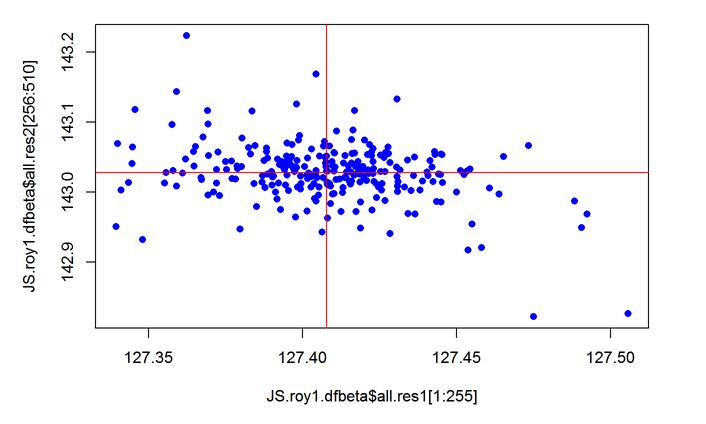
\includegraphics[width=0.7\linewidth]{images/dfbetas-JS-ROY}
		\caption{}
		\label{fig:dfbetas-JS-ROY}
	\end{figure}
	
	
	
	
	
	
	
	%---------------------------------------------------------------------------%
	%---------------------------------------------------------------------------%
	\end{document}